\documentclass[11pt]{article}

\def\dj{d\kern-0.4em\char"16\kern-0.1em}
\def\Dj{mbox{\raise0.3ex\hbox{-}\kern-0.4em D}}

\usepackage{geometry}
\usepackage{indentfirst}
\usepackage{multicol}
\usepackage{graphicx}

\geometry{
    left=10mm,
    right=60mm,
    top=20mm,
    bottom=20mm
}
\author{Lazar Vukadinovi\v c}
\date{March 29, 2016}
\title{Eratosten}

\renewcommand{\contentsname}{Sadr\v zaj}

\setlength\parskip{1em}
\linespread{1.3}

\begin{document}
    \maketitle
    \thispagestyle{empty}
    
    \newpage
    \tableofcontents
    \thispagestyle{empty}
    
    \newpage
    \pagestyle{plain}
    \setcounter{page}{1}
    \section{\v Zivot}
    
    Ro\dj en je u Kireni\footnote{danas Shahhat, Libija}, a umro u ptolomejskoj Aleksandriji. Stekao je slavu kao prvi koji je upotrebio sistem �irina i du�ina, te prvi koji je izra\v cunao Zemljinu veli\v cinu.

    \bfseries
    Eratosten se obrazovao u Aleksandriji i nekoliko godina u Atini. Ptolomej III Euergeta imenovao ga je 236. pne. predsednikom aleksandrijske biblioteke. Eratosten je dao nekoliko va�nijih doprinosa nauci. Bio je dobar prijatelj s Arhimedom. Oko 255. pne. je izumeo armilarnu sferu, koja se na�iroko koristila sve do pronalaska planetarijuma u 18. veku.

    \itshape
    Eratosten je poznat pod imenom Beta (slovo i broj 2) jer se navodno dokazao kao drugi u svetu u mnogim podru?jima. Bio je na glasu po svom bahatom karakteru. Oslepeo je 195. pne., vi�e nije mogao ?itati i godinu dana kasnije izgladneo se na smrt.\mdseries \upshape

    Eratosten je bio:
    \begin{itemize}
        \item matemati\v car
        \item astronom
        \item geograf
        \item pesnik
    \end{itemize}

    \def\figurename{slika}
    \begin{figure}[h!]
        \centering
        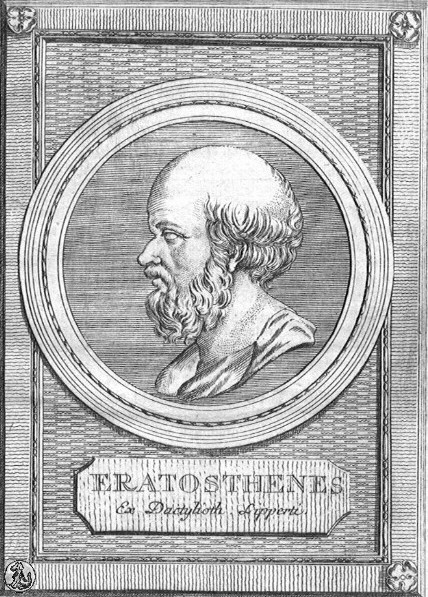
\includegraphics[width=0.5\textwidth]{Eratosthenes.jpg}
        \caption{Eratosten}
    \end{figure}

    \section{Pesni\v stvo}
    \begin{multicols}{2}
        U elegiji Erigoni pevao je ? ati?kom seljaku Ikariju, koji je prvi od Dionisa nau?io da sadi lozu, ali su ga pijani seljaci pogubili. Njegova ?erka Erigona sa svojom vernom kujom na?e le� i obesi se i, naposletku, sve troje bude uvr�teno me?u zvezde. Sli?an sadr�aj ima sa?uvani prozni spis Pretvaranja u zvezde , u kojem izla�u pri?e ? postanku sazve�?a. Delo s tim nazivom, koje imamo i koje mu se pripisuje, nije njegovo. Od njegovih dela je vrlo malo sa?uvano. Fragmenti poezije pokazuju veliku ve�tinu.

        Dok je Eratosten kao pesnik hodao putem pesnika Kalimaha, prethodnika na ?elu Biblioteke, on ga je kao istra�iva? daleko prevazi�ao. U svom velikom delu ? staroj komediji on se bavio obiljem najrazli?itijih pitanja i uticao na prou?avanja svojih naslednika Eufronija (u?itelja Aristarhovog), Aristofana i Didima.
    \end{multicols}

    \section{Odre\dj ivanje obima Zamlje}
    Oko 240. pne. Eratosten je izra?unao Zemljin opseg koriste?i se trigonometrijom i poznavanjem ugla Sun?evih zraka u odnosu na Zemlju u podne u Aleksandriji i Sieni (danas Asuan, Egipat). Ra?un je izveo pod pretpostavkom da je Zemlja okrugla i da je Sunce toliko udaljeno da se njegovi zraci mogu posmatrati kao paralelni.
    
    \newpage
    \begin{equation}
        f(x)=\left\{
        \begin{array}{rl}
            \sqrt[3]{\sqrt{\frac{x}{6}}} \cdot \log_e{4\pi}, & 0 \leq x \leq 6\\
            \lim\limits_{n \rightarrow 6}{\frac{x^2n}{n}}, & x > 6\\
            \sum\limits_{n=1}^{+\infty}{x^2 \cdot \frac{1}{n^2}}, & inace
        \end{array}
         \right.
    \end{equation}
    
\end{document}